\documentclass{eecslides}\usepackage[]{graphicx}\usepackage[]{color}
%% maxwidth is the original width if it is less than linewidth
%% otherwise use linewidth (to make sure the graphics do not exceed the margin)
\makeatletter
\def\maxwidth{ %
  \ifdim\Gin@nat@width>\linewidth
    \linewidth
  \else
    \Gin@nat@width
  \fi
}
\makeatother

\definecolor{fgcolor}{rgb}{0.345, 0.345, 0.345}
\newcommand{\hlnum}[1]{\textcolor[rgb]{0.686,0.059,0.569}{#1}}%
\newcommand{\hlstr}[1]{\textcolor[rgb]{0.192,0.494,0.8}{#1}}%
\newcommand{\hlcom}[1]{\textcolor[rgb]{0.678,0.584,0.686}{\textit{#1}}}%
\newcommand{\hlopt}[1]{\textcolor[rgb]{0,0,0}{#1}}%
\newcommand{\hlstd}[1]{\textcolor[rgb]{0.345,0.345,0.345}{#1}}%
\newcommand{\hlkwa}[1]{\textcolor[rgb]{0.161,0.373,0.58}{\textbf{#1}}}%
\newcommand{\hlkwb}[1]{\textcolor[rgb]{0.69,0.353,0.396}{#1}}%
\newcommand{\hlkwc}[1]{\textcolor[rgb]{0.333,0.667,0.333}{#1}}%
\newcommand{\hlkwd}[1]{\textcolor[rgb]{0.737,0.353,0.396}{\textbf{#1}}}%
\let\hlipl\hlkwb

\usepackage{framed}
\makeatletter
\newenvironment{kframe}{%
 \def\at@end@of@kframe{}%
 \ifinner\ifhmode%
  \def\at@end@of@kframe{\end{minipage}}%
  \begin{minipage}{\columnwidth}%
 \fi\fi%
 \def\FrameCommand##1{\hskip\@totalleftmargin \hskip-\fboxsep
 \colorbox{shadecolor}{##1}\hskip-\fboxsep
     % There is no \\@totalrightmargin, so:
     \hskip-\linewidth \hskip-\@totalleftmargin \hskip\columnwidth}%
 \MakeFramed {\advance\hsize-\width
   \@totalleftmargin\z@ \linewidth\hsize
   \@setminipage}}%
 {\par\unskip\endMakeFramed%
 \at@end@of@kframe}
\makeatother

\definecolor{shadecolor}{rgb}{.97, .97, .97}
\definecolor{messagecolor}{rgb}{0, 0, 0}
\definecolor{warningcolor}{rgb}{1, 0, 1}
\definecolor{errorcolor}{rgb}{1, 0, 0}
\newenvironment{knitrout}{}{} % an empty environment to be redefined in TeX

\usepackage{alltt}
\mode<presentation>
%\usecolortheme{BBSDark}

%%------------------
% Language and font
\usepackage[english]{babel}
\usepackage[utf8]{inputenc}

%%------------------
\usepackage{graphicx}
\usepackage{color}
\usepackage{tikz}
\usetikzlibrary{calc, shapes, backgrounds, arrows}

% --- include packages
\usepackage{subfigure}
\usepackage{multicol}
\usepackage{amsthm}
\usepackage{mathrsfs}
\usepackage{amsmath}
\usepackage{amssymb}
\usepackage{enumitem}

%%------------------
\DeclareRobustCommand\refmark[1]{\textsuperscript{\ref{#1}}}

%%------------------ Tune the template
\setbeamertemplate{blocks}[rounded][shadow=false]

\title[Day 3]{Markov Chain Monte Carlo (MCMC) and Model Evaluation}
\vspace{0.4cm}
\vspace{0.6cm}

%%% Begin slideshow
\IfFileExists{upquote.sty}{\usepackage{upquote}}{}
\begin{document}

\begin{frame}
  \titlepage
\end{frame}

\section{Introduction}


\frame{
\frametitle{Ecological context}
\framesubtitle{How important is elevation in defining sugar maple distribution on mont Sutton?}


\begin{columns}[T]
\begin{column}{0.6\textwidth}

Mont Sutton

\vspace{-0.7cm}

  \begin{center}
    \scalebox{0.2}{
      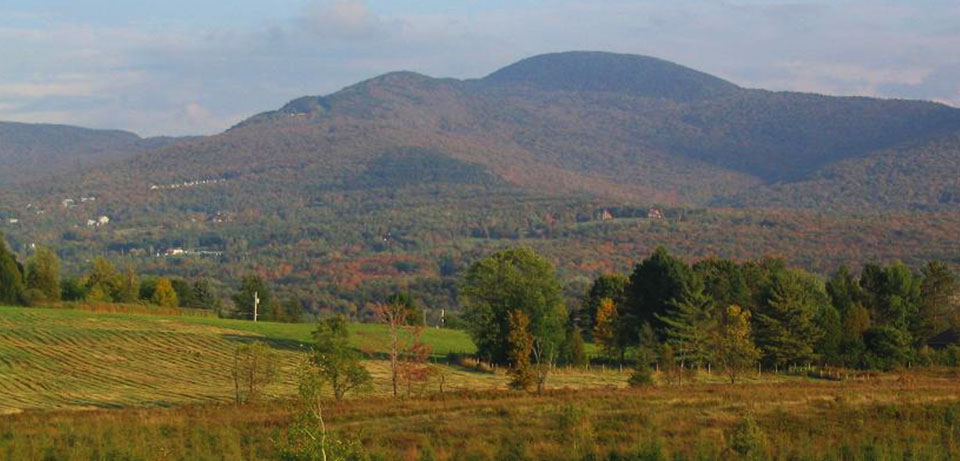
\includegraphics{Image/Mont_Sutton.jpg}
    }
  \end{center}

  \vspace{-0.2cm}
  
  {\large\bf Model}
  
  \vspace{-0.5cm}
  
  {\large $$P(y=1) = \beta x + \epsilon$$}

  \vspace{-0.8cm}

 where
 \begin{itemize}
  \item[$y$] is the distribution of sugar maple
  \item[$x$] is elevation
  \textcolor{red}{\large\item[$\beta$] is the importance of elevation}
  \item[$\epsilon$] is the model residuals
 \end{itemize}
\end{column}
\begin{column}{0.5\textwidth}
\vspace{-0.5cm}
\begin{knitrout}
\definecolor{shadecolor}{rgb}{0.969, 0.969, 0.969}\color{fgcolor}
\includegraphics[width=\maxwidth]{figure/acerSacc-1} 

\end{knitrout}
\end{column}
\end{columns}
}

\frame{
\frametitle{Linking Frequentist and Bayesian Statistics}
\framesubtitle{How can we estimate model parameters and what does it imply?}

{\Large\bf Frequentist}

\vspace{0.1cm}

%Want to find the best model parameter(s) ($\beta$) for the data at hand (sugar maple distribution)
Want to find the best model parameter(s) for the data at hand

{\Large 
	$$\textcolor{blue}{\text{Likelihood}}\hspace{1.5cm}P(\text{Data}|\text{Model})$$
}

{\large They are interested in {\bf maximizing} the \textcolor{blue}{\text{Likelihood}}}

\vspace{0.1cm}

{\large They need data}

\vspace{0.2cm}

{\bf This can be done using}

\begin{itemize}
  \item Simulated annealing
  \item The Nelder-Mead Simplex
  \item Minimizing the sums of squares
  \item \dots
\end{itemize}
}

\frame{
\frametitle{Linking Frequentist and Bayesian Statistics}
\framesubtitle{How can we estimate model parameters and what does it imply?}

{\Large\bf Bayesian}

\vspace{0.1cm}

%Want to find how good the model parameter(s) ($\beta$) given some data (sugar maple distribution)
Want to find how good the model parameter(s) are given some data

{\Large 
	$$\textcolor{orange}{\text{Posterior}}\hspace{1.5cm}P(\text{Model}|\text{Data})$$
}

{\large They are intered in the \textcolor{orange}{\text{posterior}} distribution}

\vspace{0.1cm}

{\large They need data and prior information}

\vspace{0.2cm}

{\large\bf Recall that}

{\Large 
	$$\underbrace{P(\text{Model}|\text{Data})}_{\textcolor{orange}{Posterior}}\propto \underbrace{P(\text{Data}|\text{Model})}_\text{\textcolor{blue}{Likelihood}}\underbrace{P(\text{Model})}_\text{\textcolor{green!50!black}{Prior}}$$
}

}

\frame{
\frametitle{Bayesian Statistics}
\framesubtitle{A few words about the prior}

{\Large Definition of prior probability}

\vspace{0.1cm}

The {\bf prior probability} informes us about the probability of the model being true \textit{before} the current data is considered.

\vspace{0.5cm}

{\Large Types of priors}

\vspace{0.1cm}

{\bf\large Uninformative}

\vspace{0.1cm}

These priors are meant to bring very little information about the model

\vspace{0.1cm}

{\bf\large Informative}

\vspace{0.1cm}

These priors bring information about the model that is available

}

\frame{
\frametitle{Bayesian Statistics}
\framesubtitle{A few words about the prior}

{\Large\bf Uninformative priors}

\vspace{0.1cm}

{\bf Example:} If we have no idea of how elevation influence sugar maple

\vspace{0.1cm}

{\bf Gaussian distribution}

\vspace{0.1cm}

\begin{columns}
\begin{column}{0.5\textwidth}
\large $$\frac{1}{\sqrt{2\pi\sigma^2}}e^{-\frac{(x-\mu)^2}{2\sigma^2}}$$
\end{column}
with
\begin{column}{0.5\textwidth}
\begin{itemize}
  \item $\mu = 0$
  \item $\sigma = \text{Large say 100}$
\end{itemize}
\end{column}
\end{columns}

\vspace{0.2cm}
\begin{knitrout}
\definecolor{shadecolor}{rgb}{0.969, 0.969, 0.969}\color{fgcolor}
\includegraphics[width=\maxwidth]{figure/uninfoPrior-1} 

\end{knitrout}

}

\frame{
\frametitle{Bayesian Statistics}
\framesubtitle{A few words about the prior}

{\Large\bf Informative priors}

\vspace{0.1cm}

{\bf Example:} If we know that 
\begin{itemize}
  \item There are less sugar maples the higher we go
  \item The influence of elevation on sugar maple cannot be more than two folds
\end{itemize}

\vspace{0.1cm}

{\bf Uniform distribution}

\vspace{0.1cm}

\begin{columns}
\begin{column}{0.5\textwidth}
\large $$\left\{
  \begin{array}{cl}
    \frac{1}{b-a} & \text{for } x\in [a,b]\\
    0 &\text{otherwise}\\
  \end{array}
\right.$$
\end{column}
with
\begin{column}{0.5\textwidth}
\begin{itemize}
  \item $a > -2$
  \item $b < 0$
\end{itemize}
\end{column}
\end{columns}

\vspace{0.2cm}
\begin{knitrout}
\definecolor{shadecolor}{rgb}{0.969, 0.969, 0.969}\color{fgcolor}
\includegraphics[width=\maxwidth]{figure/infoPrior-1} 

\end{knitrout}
}


\section{Bayesian}

\frame{
\frametitle{Bayesian Statistics}
\framesubtitle{Estimating model parameters}

{\large\bf When the likelihood \textit{can} be solved analytically}

\vspace{0.2cm}

{\bf Example}

\vspace{0.1cm}

Assuming that the sugar maple follows a binomial distribution where

\begin{itemize}[leftmargin=2cm]
  \item[Data:] $y$
  \item[Model ($\theta$):] $\beta x$
\end{itemize}
then the \textcolor{blue}{likelihood} is
\begin{align*}
  P(y|\theta)&=\binom{1}{y}\theta^y\left(1-\theta\right)^{1-y}\\
  &\propto\theta^y\left(1-\theta\right)^{1-y}\\
  &\propto\left(\beta x\right)^y\left(1-\beta x\right)^{1-y}\\
\end{align*}


}

\frame{
\frametitle{Bayesian Statistics}
\framesubtitle{Estimating $\beta$}
Exercice (by hand?)
}

\frame{
\frametitle{Bayesian Statistics}
\framesubtitle{Estimating $\beta$}

{\Large When the likelihood {\bf cannot} be solved analytically (Difficult problem)}

Talk about MCMC
Mention that MCMC {\bf can} be used for simple problems but it is generally time consumming so generally not the best way to go
}

\section{MCMC}

\frame{
\frametitle{The general concepts underlying Markov Chain Monte Carlo (MCMC)}

Link with simulated annealing
}

\section{Metropolis-Hasting}

\frame{
\frametitle{The Metropolis-Hasting Algorithm}
Present a detailled example of the algorithm
}

\subsection{Adaptive Metropolis}

\frame{
\frametitle{The Adaptive Metropolis Algorithm}
Show what needs to be added to make MA adaptative

show how this helps with the example

}

\subsection{SCAM}

\frame{
\frametitle{The Single Component Adaptive Metropolis Algorithm}
Show what needs to be added to make MA a SCAM

show how this helps with the example
}

\frame{
\frametitle{The Single Component Adaptive Metropolis Algorithm with Rotation}
Show what needs to be added to make MA a SCAM

show how this helps with the example
}

\frame{
\frametitle{Gibbs Sampling}
Gibbs sampling is a special case of MA

Show an example of how this works

This is particularly useful for hierarchical models
}

\frame{
\frametitle{Metropolis-Hastings }
Exercice: Build your own for a one parameter model
}

\frame{
\frametitle{Metropolis-Hastings \& Gibbs sampler}
Exercice: Build your own for a two parameter model
}

\section{Diagnostics}
\subsection{Visual}

\frame{
\frametitle{Trace plot}

}

\frame{
\frametitle{Density plot}

}

\frame{
\frametitle{Trace plot}
Exercice: Build your own and compare it to the one of \texttt{coda}

}

\subsection{Statistics}

\frame{
\frametitle{Gelman and Rubin's convergence diagnostics}

}

\frame{
\frametitle{Geweke's convergence diagnostics}

}

\frame{
\frametitle{Heidelberger and Welch's convergence diagnostics}

}

\frame{
\frametitle{Raftery and Lewis's convergence diagnostics}

}

\section{Good Practices}

\frame{
\frametitle{Number of runs}

}
\frame{
\frametitle{Number of iterations}

}

\frame{
\frametitle{Burning}

}

\frame{
\frametitle{Thinning}

}


\end{document}
